\begin{figure}[H]
\centering
\subfloat[$a = 0$, $b = 1$]{
  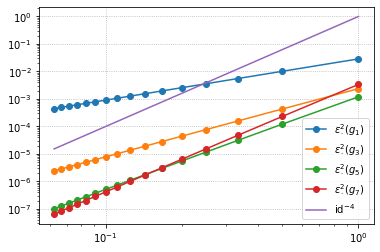
\includegraphics[width=65mm]{Aufgabe_2/latex_code/images/konvergenz_plot_2_1.png}
}
\subfloat[$a = \frac{1}{2}$, $b = 1$]{
  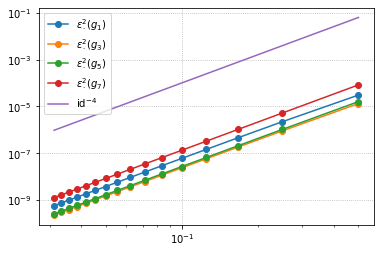
\includegraphics[width=65mm]{Aufgabe_2/latex_code/images/konvergenz_plot_2_2.png}
}
\hspace{0mm}
\caption{Konvergenzverhalten von $\epsilon_\cdot^{(2)}(g_k)$, $k = 1, 3, 5, 7$ auf $[a, b]$}
\label{fig:konvergenz_plot_2}
\end{figure}